\documentclass[12pt, letterpaper]{article}
\usepackage{babel}
\usepackage[T1]{fontenc}
\usepackage{textcomp}
\usepackage[utf8]{inputenc} % Puede depender del sistema o editor
\usepackage{amsmath}
\usepackage{amsfonts}
\usepackage{amssymb}
\usepackage[left=2cm,right=2cm,top=2cm,bottom=2cm]{geometry}
\usepackage{mathrsfs}
\usepackage{pstricks-add}
\usepackage{pgfkeys}
\usepackage{setspace}
\usepackage{fancyhdr}
\usepackage{graphicx}
\usepackage{enumerate}

\usepackage{tikz}
\usetikzlibrary{fit,positioning}
\begin{document}
\begin{titlepage}
	\centering
	{\scshape\LARGE Instituto Politécnico Nacional\\ Unidad Profesional Interdisiplinaria de Ingenierias campus Zacatecas\par}
	\vspace{1cm}
	{\scshape\Large Probabilidad Y Estadistica\par}
	\vspace{1.5cm}
	{\huge\bfseries Unidad 2 Tarea 2\par}
	\vspace{2cm}
	{\Large\itshape Olando Odiseo Belmonte Flores\par}
	\vfill
	Maestro:\par
	\textsc{
	Rosendo Vasquez Bañuelos}
	\vfill
% Bottom of the page
	{\large \today \par}
\end{titlepage}

\textbf{2} Suponga que la temperatura de reaccion $X$ (en °C) en cierto proceso químico tiene una distribución uniforme con $A=-5$ y $B=5$
\begin{enumerate}[a)]
    \item calule $P(X<0)$\\
		$f(x)=\left\{\begin{array}{l c}
			\displaystyle\frac{1}{10},& si\ x\in (A,B)\\ \\
			0 & en\ otro\ caso
		\end{array}\right.
		$\vskip0.1cm
		$F(x)=\displaystyle\int_{-5}^{x}\displaystyle\frac{1}{10}dt=\displaystyle\frac{1}{10}\int_{-5}^{x}dt = \left.\frac{t}{10} \right|_{-5}^x=\displaystyle\frac{x+5}{10}$\vskip0.1cm
		$P(X<0)=\displaystyle\frac{0+5}{10}-\displaystyle\frac{(-5)+5}{10}=\displaystyle\frac{5}{10}=0.5$

	\item Calcule $P(-2.5<X<2.5)$\vskip0.1cm
		$P(-2.5<X<2.5)=\displaystyle\frac{2.5+5}{10}-\displaystyle\frac{(-2.5)+5}{10}=\displaystyle\frac{7.5-2.5}{10}=\displaystyle\frac{5}{10}=0.5$

	\item Calcule $P(-2\leq X\leq 3)$\vskip0.1cm
		$P(-2\leq X\leq 3)=\displaystyle\frac{3+5}{10}-\displaystyle\frac{(-2)+5}{10}=\displaystyle\frac{8-3}{10}=\displaystyle\frac{5}{10}=0.5$

	\item Para que $k$ satisfaga $-5<k<k+4<5$, calcule $P(k<X<k+4)$\vskip0.1cm
	$P(k<X<k+4)=\displaystyle\frac{(k+4+5)-(k+5)}{10}=\displaystyle\frac{k+4+5-k-5}{10}=\displaystyle\frac{4}{10}=0.4$
\end{enumerate} \vskip1cm

\textbf{4} Sea $X$ el esfuerzo vibratorio($lb/pulg^2$) en el aspa de una turbina de viento a una velocidad del viento particular en un túnel aerodinámico. El árticulo \textit{"Blade Fatigue Life Assessment with Applications to VAWTS" (J. Solar Energy Enrg. 1982: 107-111)} propone la distribución Rayleigh, con función de densidad de probabilidad\vskip0.1cm
$f(x;0)=\left\{\begin{array}{l c}
	\displaystyle\frac{x}{\theta ^2}\centerdot e^{-x^2/2\theta ^2}, & x>0\\ \\
	0 & de\ lo\ contrario
\end{array}\right.$\vskip0.5cm
como modelo de la distribucion de $X$.\vskip0.5cm
\begin{enumerate}[a)]
	\item Verifique  que $f(x;\theta)$ es una funcion de dencidad de probabilidad legitima\\
		$\displaystyle\int_0^\infty\displaystyle\frac{x}{\theta^2}e^{\frac{-x^2}{2\theta^2}}dx=\displaystyle\frac{1}{\theta^2}\lim_{t\to\infty}\int_0^txe^udu$
		$\begin{array}{l c}
			Sea\ u=\displaystyle\frac{-x^2}{2\theta^2} & du = \displaystyle\frac{-x}{\theta^2}dx\\
		 	& xdx=-\theta^2du
		\end{array}$\vskip0.1cm
		$=\displaystyle\frac{1}{\theta^2}\lim_{t\to\infty}\int_0^t-\theta^2e^udu=\displaystyle\frac{-\theta^2}{\theta^2}\lim_{t\to\infty}\int_0^te^udu=-\left.\lim_{t\to\infty}e^u\right|_0^t=-\left.\lim_{t\to\infty}e^{\frac{-x^2}{2\theta^2}}\right|_0^t$\vskip0.1cm$=-\displaystyle\lim_{t\to\infty}\left[e^{\frac{-t^2}{2\theta^2}} - e^{\frac{-0^2}{2\theta^2}}\right]=-(-1)=1$
	\item Suponga que $\theta = 100$ (un valor sugerido por una gráfica en el artículo). ¿Cuál es la probabilidad de que $X$ es cuando mucho de $200$?¿Menos de $200$?¿Por lo menos de 200?\vskip0.1cm
		$F(x) = \displaystyle\int_0^x\frac{t}{\theta^2}e^{\frac{-t^2}{2\theta^2}}dt=1+e^{\frac{-x^2}{2\theta^2}}$\\
		$P(x\leq200;\theta=100) = 1-e^{\frac{-(200^2)}{2(100^2)}}=1+e^{\frac{-40000}{20000}}=1-e^{-2}=0.8646$\vskip0.1cm
		$P(x<200;\theta=100) = 1-e^{\frac{-(200^2)}{2(100^2)}}=1+e^{\frac{-40000}{20000}}=1-e^{-2}=0.8646$\vskip0.1cm
		$P(x\geq200;\theta=100)=\left(1-e^{\frac{-\infty}{20000}}\right) - \left(1+e^{\frac{-40000}{20000}} \right) = 1 + e^{-2} - 1 = 0.1353$
	\item ¿Cuál es la probabilidad de que $X$ esté entre $100$ y $200$ (de nuevo con $\theta=100$)?\vskip0.01cm
		$P(100<X<200;\theta=100)=\left(1-e^{\frac{-(200^2)}{2(100^2)}}\right)-\left(1-e^{\frac{-100^2}{2(100^2)}}\right)=e^{\frac{-1}{2}}-e^{\frac{-40000}{20000}}+1-1=e^{\frac{-1}{2}}-e^{-2}=0.4711$
	\item De una expresión para $P(X\leq x)$\vskip0.01cm
		$\displaystyle\int_0^x\frac{t}{\theta^2}e^{\frac{-t}{2\theta^2}}dt=\displaystyle\frac{1}{\theta^2}\int_0^xte^{\frac{-t}{2\theta^2}}dt$
		$\begin{array}{l c}
			Sea\ u=\displaystyle\frac{-t^2}{2\theta^2} & du = \displaystyle\frac{-t}{\theta^2}dt\\
		 	& tdt=-\theta^2du
		\end{array}$\vskip0.1cm
		$\left.\displaystyle\frac{-\theta^2}{\theta^2}\int_0^xe^udu?-\displaystyle\int_0^xe^udu=-e^u\right|_0^x=\left.-e^{\frac{-t}{2\theta^2}}\right|_0^x=-e^{\frac{-x}{2\theta^2}}-(-e^{\frac{-0^2}{2\theta^2}})=1-e^{\frac{-x^2}{2\theta^2}}$

\end{enumerate}
\vskip1cm

\textbf{6} El peso de lectura real de una pastilla de etéreo ajustado a 3 gramos en un tocadiscos particular puede ser considerado como na variable aleatoria continua $X$ con función de densidad de probabilidad
$f(x)=\left\{\begin{array}{c l}
	k[1-(x-3)^2], & 2\leq x\leq 4\\
	0, & de\ lo\ contrario
\end{array}\right.$
\begin{enumerate}[a)]
	\item Trace la graic de $f(x)$\vskip0.1cm
	\begin{center}
		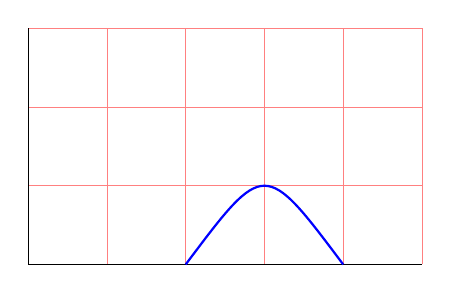
\begin{tikzpicture}
			\draw[step=1,color=red!50!white, very thin] (0,0)
			grid (5,3);
			\draw (0,0) -- (5,0);
			\draw (0,0) -- (0,3);
			\draw[thick, color=blue] (2,0) .. controls (3,1.333) .. (4,0);
		\end{tikzpicture}
	\end{center}
	\item Determine ek valor de $k$\vskip0.1cm
		$\displaystyle\int_2^4k[1-(x-3)^2]dx=k\int_2^4dx-k\int_2^4(x-3)^2dx=k\left[\int_2^4dx-\int_2^4x^2dx+6\int_2^4xdx-9\int_2^4dx\right]=k\left[-\int_2^4x^2dx+6\int_2^4xdx-8\int_2^4dx \right]=$
		$k\left[\left.\displaystyle\frac{x^3}{3}+3x^2-8x  \right]\right|_2^4= k\left[\displaystyle\frac{-(4^3-2^3)}{3}+3(4^2-2^2)-8(4-2) \right] = k\left[\displaystyle\frac{-56}{3}+36-16 \right]=\displaystyle\frac{4}{3}k=1$\vskip0.1cm
		$k=\displaystyle\frac{3}{4}$
	\item ¿Cuál es la probabiliad de que el peso real de lectura sea mayor que el peso prescrito?\vskip0.1cm
		$P(3<X<4)=\displaystyle\frac{3}{4}\int_3^4[1-(x-3)^2]dx=\frac{3}{4}\left[-\int_3^4x^2dx+6\int_3^4xdx-8\int_3^4dx\right]=\frac{3}{4}\left[\left.-\frac{x^3}{3}+3x^2-8x \right]\right|_3^4$
		$\displaystyle\frac{3}{4}\left[\frac{-(4^3-3^3)}{3}+3(4^2-3^2)-8(4-3)\right]=\frac{3}{4}\centerdot \frac{2}{3}=\frac{1}{2}=0.5$
	\item ¿Cuál es la probabilidad de que el peso real de lectura esté dentro de 0.25 gramos el peso prescrito?\vskip0.1cm
		$P(2.25<X<3)=\displaystyle\frac{3}{4}\int_{2.25}^3[1-(x-3)^2]dx=\frac{3}{4}\left[-\int_{2.25}^3x^2dx+6\int_{2.25}^3xdx-8\int_{2.25}^3dx\right]=\frac{3}{4}\left[\left.-\frac{x^3}{3}+3x^2-8x \right]\right|_{2.25}^3$
		$\displaystyle\frac{3}{4}\left[\frac{-(3^3-2.5^3)}{3}+3(3^2-2.5^2)-8(3-2.5)\right]=\frac{3}{4}\centerdot \frac{607}{1000}$\vskip0.1cm
		$=\displaystyle\frac{1821}{4000}=0.455$
	\item ¿Cuál es la probabilidad d eque el peso real difiera del peso prescrito por más de 0.5 gramos?\vskip0.1cm
	$P(3.5<X<4)=\displaystyle\frac{3}{4}\int_{3.5}^4[1-(x-3)^2]dx=\frac{3}{4}\left[-\int_{3.5}^4x^2dx+6\int_{3.5}^4xdx-8\int_{3.5}^4dx\right]=$\vskip0.1cm
	$\displaystyle\frac{3}{4}\left[\left.-\frac{x^3}{3}+3x^2-8x \right]\right|_{3.5}^4$
	$\displaystyle\frac{3}{4}\left[\frac{-(4^3-3.5^3)}{3}+3(4^2-3.5^2)-8(4-3.5)\right]=\frac{3}{4}\centerdot \frac{26}{125}=\frac{78}{500}$\vskip0.1cm
	$=\displaystyle\frac{39}{250}=0.156$
\end{enumerate}\vskip1cm

\textbf{8} Para ir al trabajo primero tengo que tomar un camión cerca de mi casa y luego tomar un segundo camión. Si el tiempo de espera (en minutos) en cada parada tiene una distribución uniforme con $A=0$ y $B=5$, entonces se puede demostrar que el tiempo de espea total $Y$ tiene una función de densidad de probabilidad\vskip0.1cm
$f(x)=\left\{\begin{array}{c l}
	\displaystyle\frac{1}{25}y, & 0\leq y<5\\\\
	\displaystyle\frac{2}{5}-\frac{1}{25}y, & 5\leq y\leq 10\\\\
	0, & y<0\ o\ y>10
\end{array}\right.$
\begin{enumerate}[a)]
	\item Trace a gráfica de la función dedensdad de probabilidad de $Y$\vskip0.1cm
	\begin{center}
		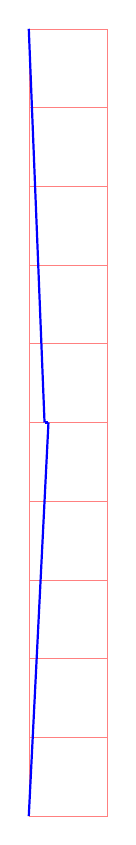
\begin{tikzpicture}
			\draw[step=1,color=red!50!white, very thin] (0,0)
			grid (1,10);
			\draw[thick, color=blue] (0,0) -- (0.25,5);
			\draw[thick, color=blue] (0.2,5) --  (0.25,5);
			\draw[thick, color=blue] (0.2,5) --  (0,10);

		\end{tikzpicture}
	\end{center}
	\item Verifique que $\displaystyle\int_{-\infty}^\infty f(y)dy=1$\\
		$\displaystyle\int_0^5\frac{1}{25}ydy+\int_5^{10}\left[\frac{2}{5}-\frac{1}{25}y \right]dy=\frac{1}{25}\int_0^5ydy-\frac{1}{25}\int_5^{10}ydy+\frac{2}{5}\int_5^{10}dy=\left.\frac{y^2}{50}\right|_0^{5}- \left.\frac{y^2}{50}\right|_5^{10}+\left.\frac{2}{5}y\right|_5^{10}$\vskip0.1cm
		$=\displaystyle\frac{25}{50}-\frac{100-25}{50}+\frac{20-10}{5}=\frac{1}{2}-\frac{3}{2}+\frac{10}{5}=\frac{-2}{2}+2=-1+2=1$
	\item ¿Cuál es la probabulidad  de que el tiempo de espera total sea cuando mucho de tres minutos?\\
		$P(y\leq 3)=\displaystyle\int_0^3\frac{1}{25}ydy=\frac{1}{25}\int_0^3ydy=\left.\frac{y^2}{25}\right|_0^3=\frac{9}{50}=0.18$
	\item ¿Cuál es la probabilidad de que el tiempo de espera total sea de cuando mucho de ocho minutos?\\
		$P(y\leq 8)=\displaystyle\int_0^5\frac{1}{25}ydy+\int_5^8\left[\frac{2}{5}-\frac{1}{25}y \right]dy=\frac{1}{25}\int_0^5ydy-\frac{1}{25}\int_5^8ydy+\frac{2}{5}\int_5^8dy$\vskip0.1cm
		$=\displaystyle\left.\frac{y^2}{50}\right|_0^5- \left.\frac{y^2}{50}\right|_5^8+\left.\frac{2}{5}y\right|_5^8=\frac{25}{50}-\frac{39}{50}+\frac{6}{5}=\frac{6}{5}-\frac{14}{50}=\frac{23}{25}=0.92$
	\item ¿Cuál es la probabilidad de que el tiempo de espera total sea de cuadno esté entre tres y ocho minutos?\\
		$P(3\leq y\leq 8)=\displaystyle\int_3^5\frac{1}{25}ydy+\int_5^8\left[\frac{2}{5}-\frac{1}{25}y \right]dy=\frac{1}{25}\int_3^5ydy-\frac{1}{25}\int_5^8ydy+\frac{2}{5}\int_5^8dy$\vskip0.1cm
		$=\displaystyle\left.\frac{y^2}{50}\right|_3^5- \left.\frac{y^2}{50}\right|_5^8+\left.\frac{2}{5}y\right|_5^8=\frac{16}{50}-\frac{39}{50}+\frac{6}{5}=\frac{6}{5}-\frac{23}{50}=\frac{37}{50}=0.74$
	\item ¿Cuál es la probabilidad de que el tiempo de esperatotal sea de menos de 2 minutos o de mas de 6 minutos?\\
	$P(y<2,y>6)=\displaystyle\int_0^2\frac{1}{25}ydy+\int_6^{10}\left[\frac{2}{5}-\frac{1}{25}y \right]dy=\frac{1}{25}\int_0^2ydy-\frac{1}{25}\int_6^{10}ydy+\frac{2}{5}\int_6^{10}dy$\vskip0.1cm
	$=\displaystyle\left.\frac{y^2}{50}\right|_0^2- \left.\frac{y^2}{50}\right|_6^{10}+\left.\frac{2}{5}y\right|_6^{10}=\frac{4}{50}-\frac{64}{50}+\frac{8}{5}=\frac{8}{5}-\frac{60}{50}=\frac{2}{5}=0.4$
\end{enumerate}\vskip1cm

\textbf{10} Una familia de funciones de densidad de probabilidad que ha sido utilizada para aproximar la disribución del ingreso, el tamaño de la población de una ciudad y el tamaño de firmas es de la familia Pareto. La familia tine dos parametros $k$y $\theta$, ambos $>0$ y la funcion de densidad de probabilidad es\vskip0.1cm
$f(x)=\left\{\begin{array}{c l}
	\displaystyle\frac{k\theta^k}{x^{k+1}}, & x>\theta\\ \\
	0, & x<\theta
\end{array}\right.$
\begin{enumerate}[a)]
	\item trace la grafica de $f(x;k,\theta)$\vskip0.1cm
	\begin{center}
		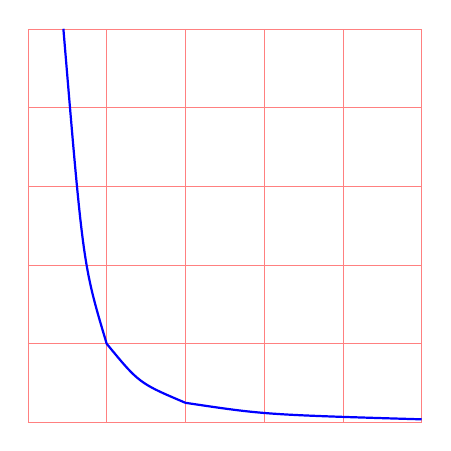
\begin{tikzpicture}
			\draw[step=1,color=red!50!white, very thin] (0,0)
			grid (5,5);
			\draw[thick, color=blue] (0.45,5) .. controls (0.7,2) .. (1,1) .. controls (1.411,0.5) ..  (2,0.25) .. controls (3,0.1) .. (5,0.04);
		\end{tikzpicture}
	\end{center}
	\item Verifique que el área total bajo la grafica es igual a $1$\vskip0.1cm
		$\displaystyle\int_\theta^\infty\frac{k\theta^k}{x^{k+1}}dx=k\theta^k\lim_{t\to \infty}\int_\theta^t\frac{1}{x^{k+1}}dx=\left.k\theta^k\lim_{t\to \infty}\frac{1}{-kx^k}\right|_\theta^t=k\theta^k\lim_{t\to \infty}\left[\frac{1}{-kt^k}-\frac{1}{-k\theta^k}\right]=\frac{-k\theta^k}{-k\theta^k}=1$
	\item Si la variable aleatoria $X$ tiene una funcion de densidad de probabilidad $f(x;k,\theta)$, con cualquier $b>\theta$, obtenga una exprecion para $P(X\leq b)$\vskip0.1cm
		$P(X\leq b)=\displaystyle\int_\theta^b\frac{k\theta^k}{x^k+1}dx=k\theta^k\int_\theta^b\frac{1}{x^{k+1}}dx=\left.\frac{k\theta^k}{-kx^k}\right|_\theta^b=\left.\frac{\theta^k}{-x^k}\right|_\theta^b=\frac{\theta^k}{-b^k}-\frac{\theta^k}{-\theta^k}=1+\frac{\theta^k}{-b^k}$
	\item Con $\theta<a<b$, obtenga una expresión para la probabilidad $P(a\leq X\leq b)$\vskip0.1cm
		$P(a\leq X\leq b)=\displaystyle\int_a^b\frac{k\theta^k}{x^k+1}dx=k\theta^k\int_a^b\frac{1}{x^{k+1}}dx=\left.\frac{k\theta^k}{-kx^k}\right|_a^b=\left.\frac{\theta^k}{-x^k}\right|_a^b=\frac{\theta^k}{-b^k}-\frac{\theta^k}{-a^k}=\frac{\theta^k}{a^k}+\frac{\theta^k}{-b^k}$, $\theta<a<b$
\end{enumerate}
\end{document}
